\section{Experiments and Results}

This research evaluated segmentation and classification tasks using the MRI brain datasets. All images were standardized to a 2D format and underwent normalization to ensure consistency in pixel intensity and reduce variations from acquisition conditions. 

Using roto-translation equivariance combined with 2.5D spatial context and Edge-Boundary loss, the upgraded Mod-SE(2) demonstrated improved spatial consistency and reduced false positives, validating its robustness in clinical imaging tasks. We evaluated our architecture using a rigorous slice-level 10-fold cross-validation scheme to ensure statistical validity.

\subsection{Qualitative Analysis}
Figure~\ref{fig:heatmap} displays the predicted heatmaps of our model across three different brain slices, highlighting the model's high confidence within the tumor core and precise boundary delineation. 

\begin{figure}[h]
    \centering
    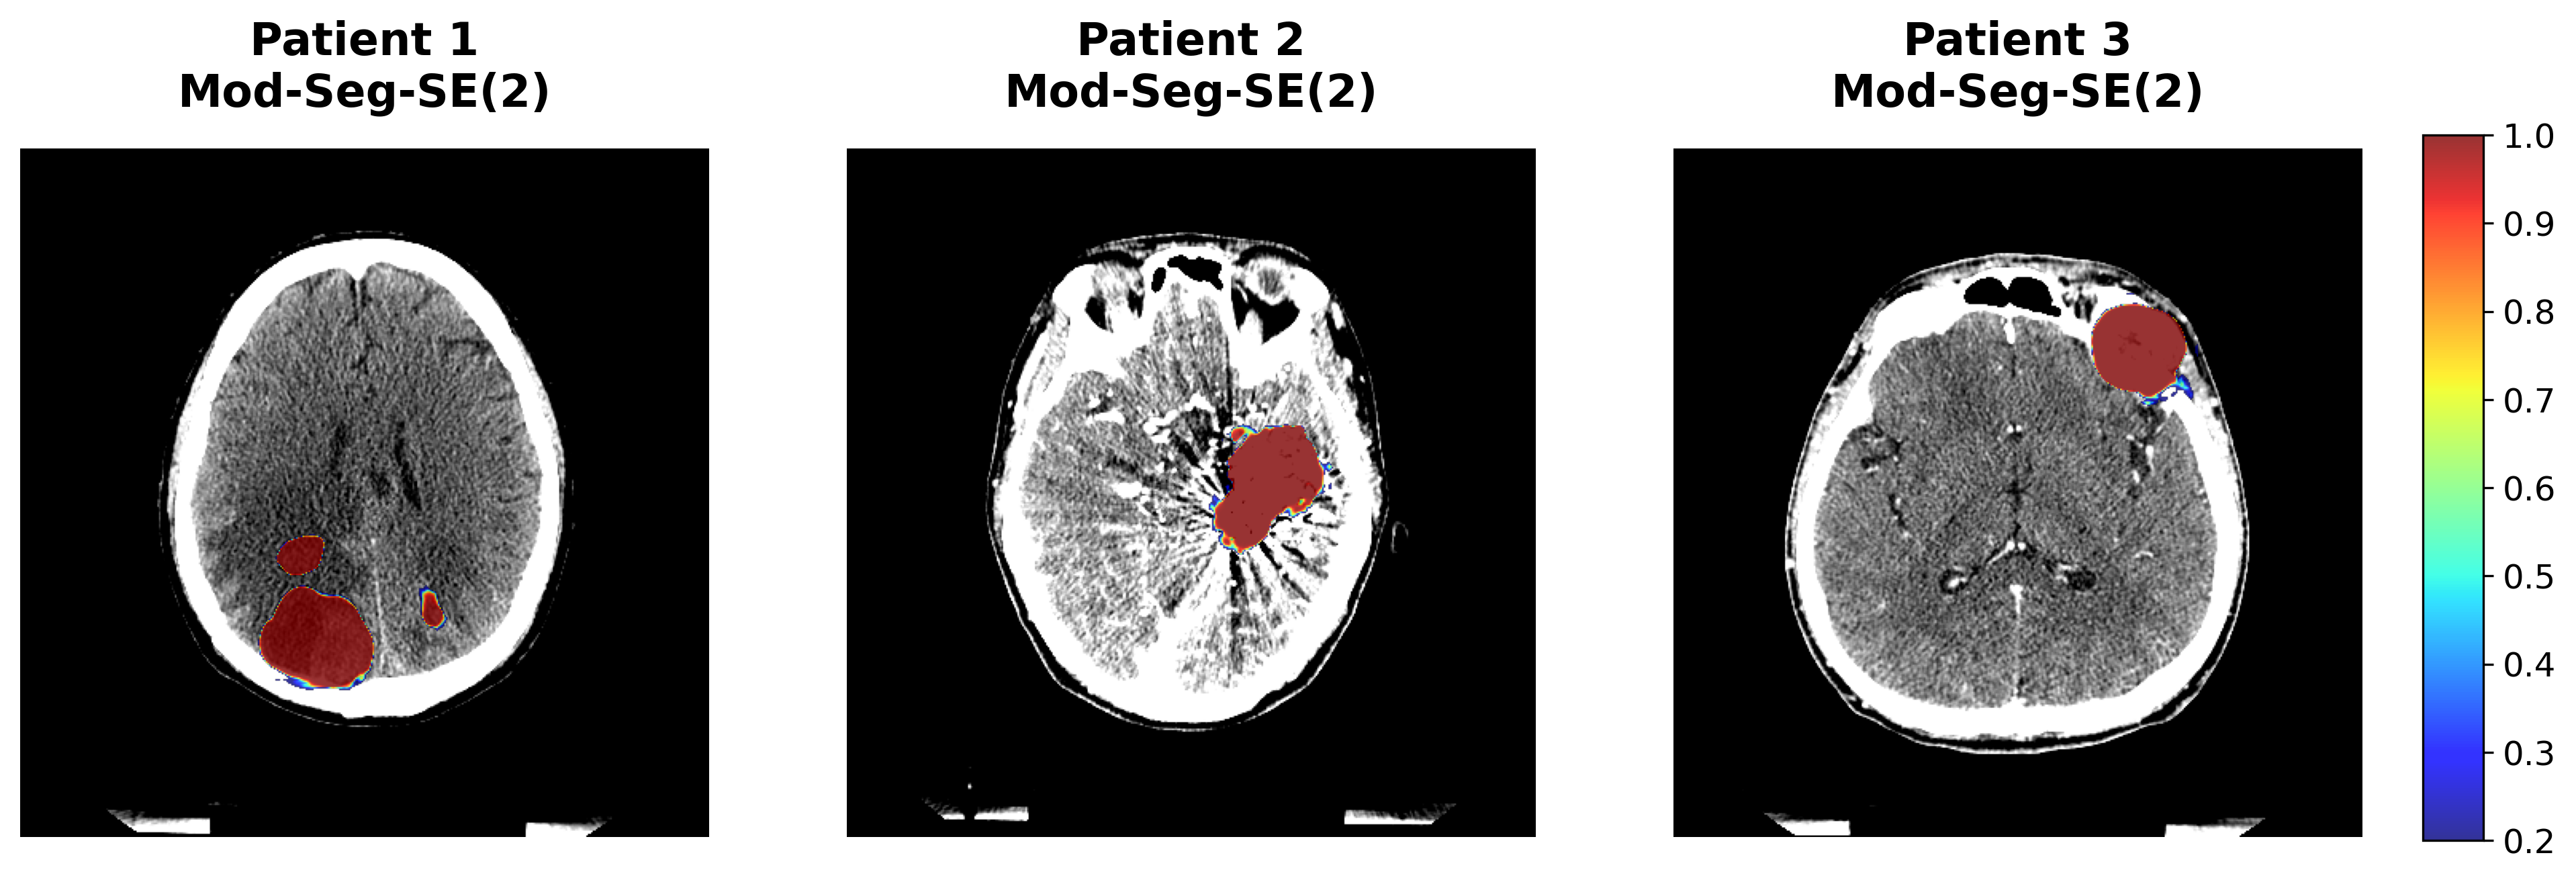
\includegraphics[width=\linewidth]{Journal_Figures/Fig1_3Brain_Heatmap_Journal.png}
    \caption{Qualitative heatmaps demonstrating the model's confidence across three distinct tumor topologies. Mod-SE(2) demonstrates accurate and focused segmentation.}
    \label{fig:heatmap}
\end{figure}

Furthermore, Figure~\ref{fig:grid} provides a direct visual comparison between the ground truth masks and our model's predictions, showcasing the efficacy of the Edge-Boundary Loss in preventing over-segmentation along the ambiguous margins. This is critical for neurosurgical planning, where overestimating tumor bounds can lead to resection of healthy tissue.

\begin{figure}[h]
    \centering
    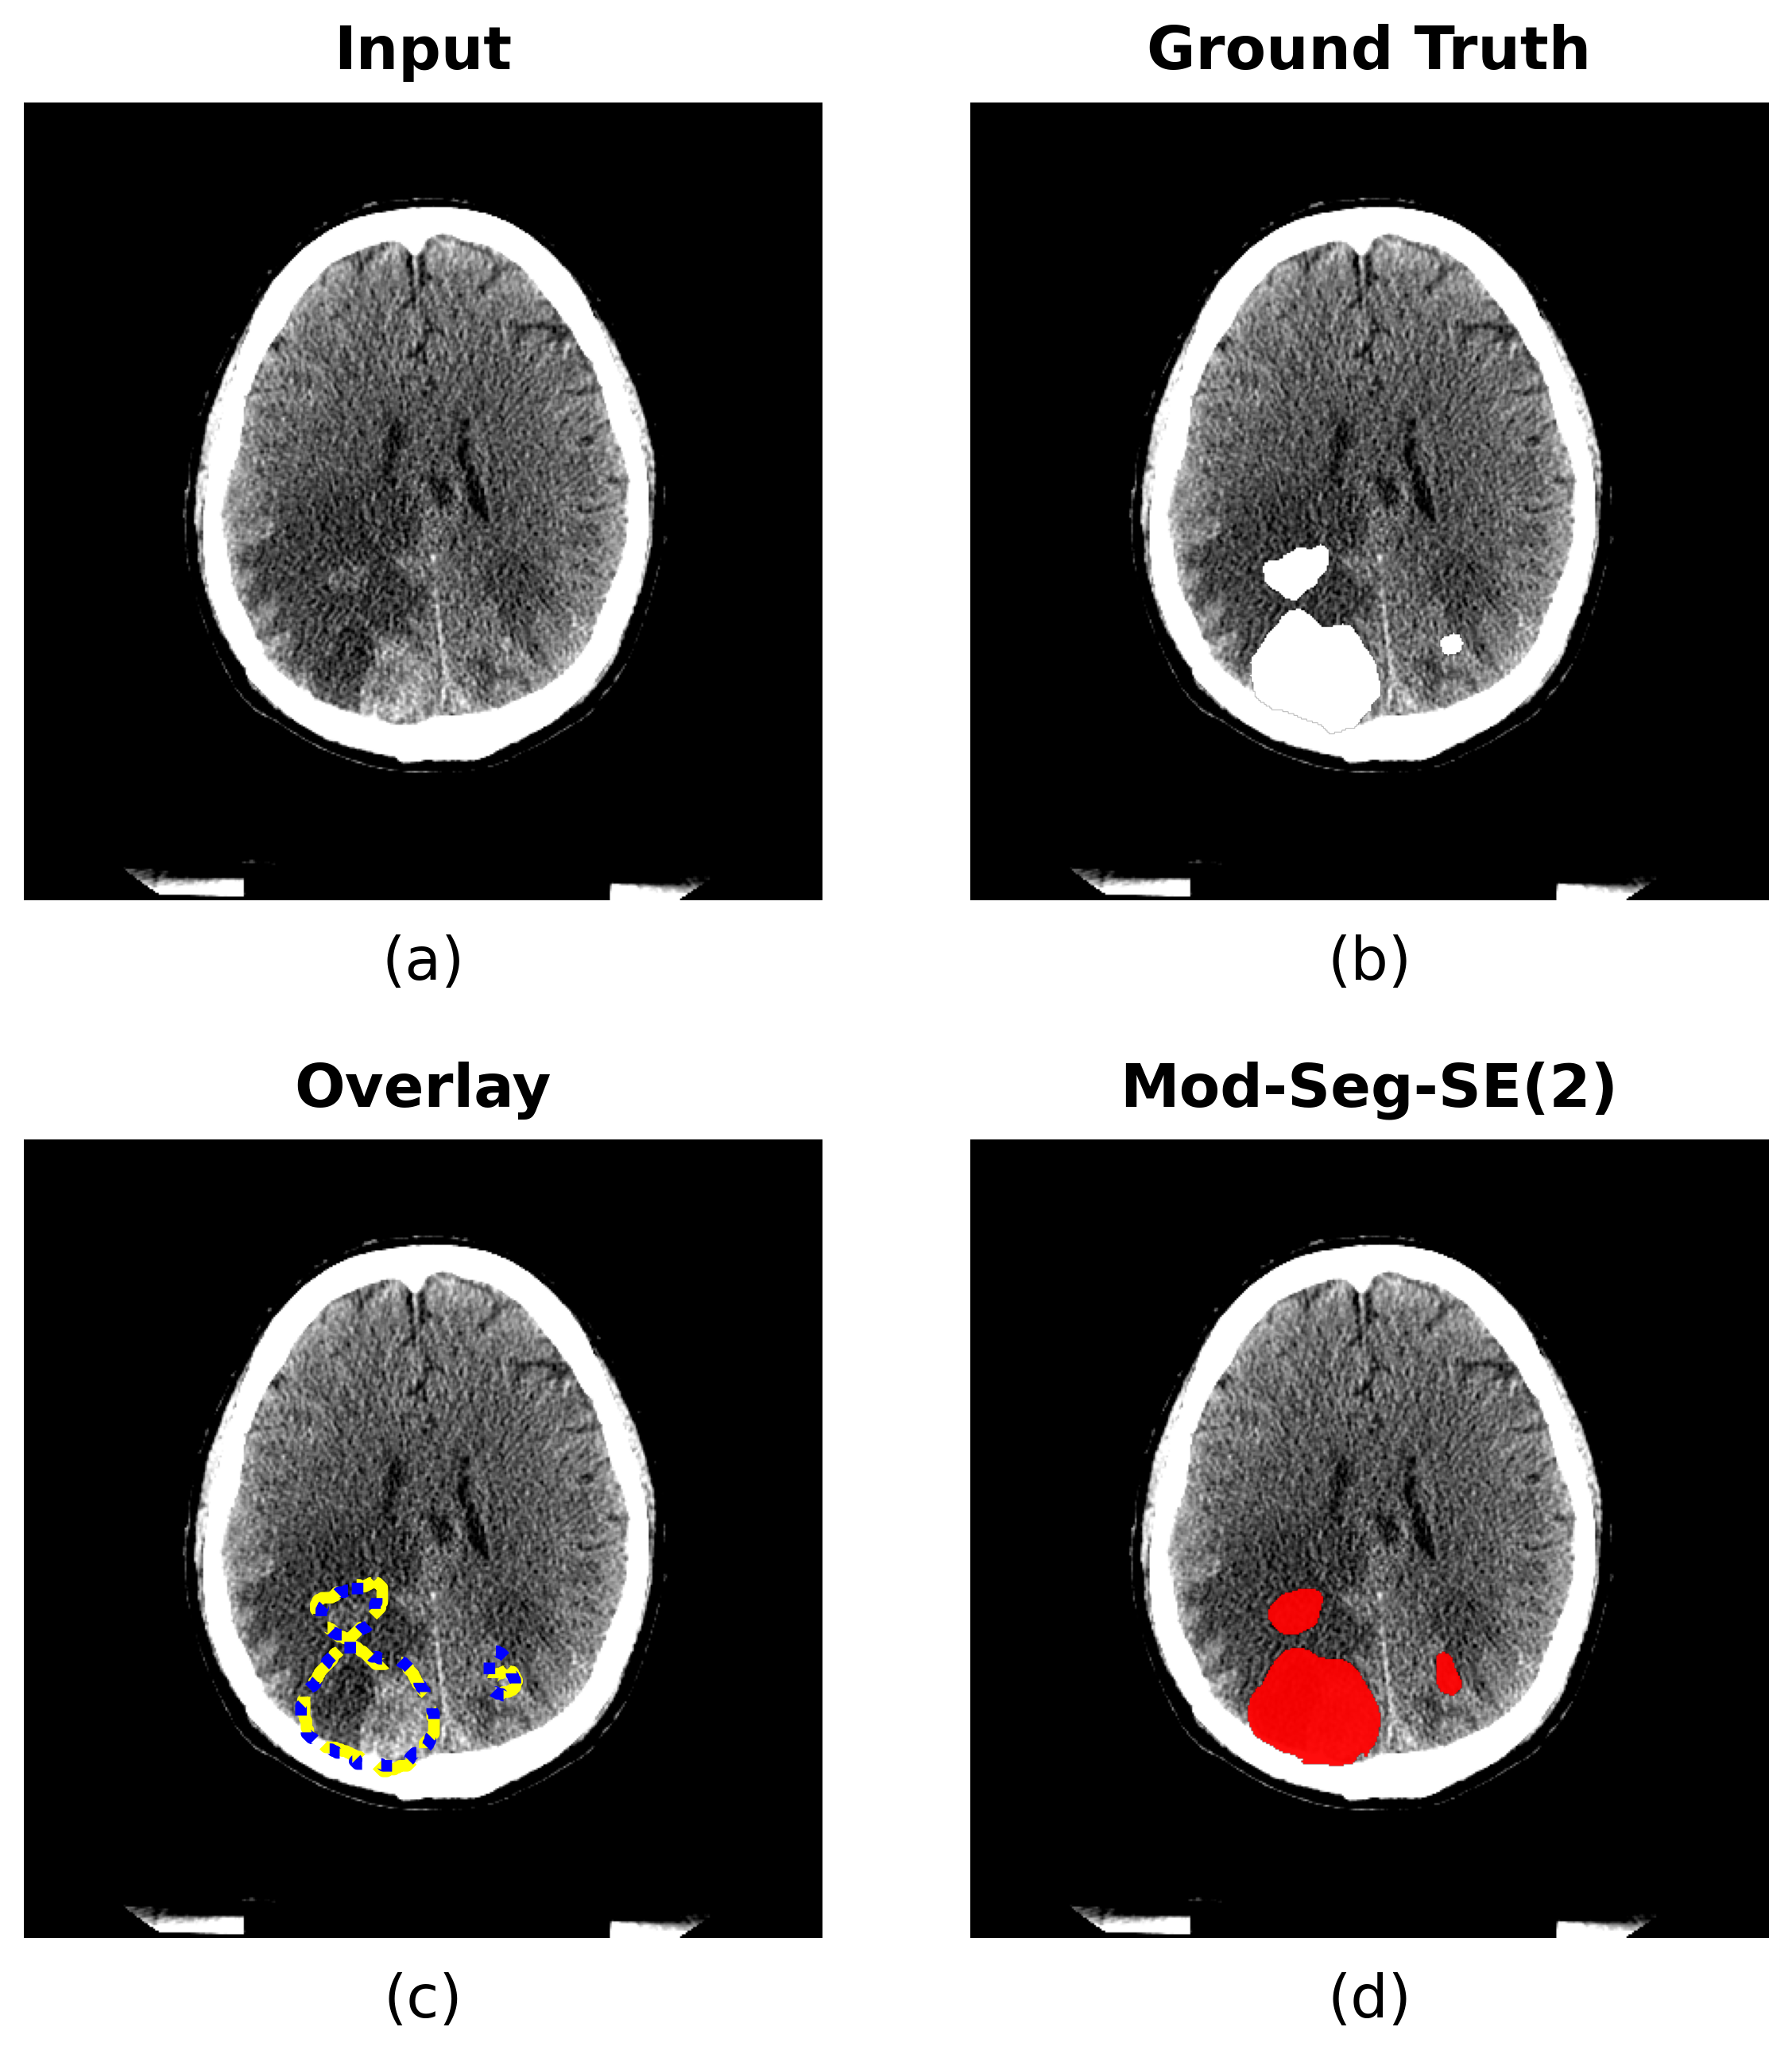
\includegraphics[width=\linewidth]{Journal_Figures/Fig2_Segmentation_Grid.png}
    \caption{Comparative segmentation grid showing the original CT, Ground Truth, and SE2-CNNET Prediction.}
    \label{fig:grid}
\end{figure}

\subsection{Quantitative Analysis}
Our comprehensive evaluation metrics validate the proposed architectural improvements. The model achieves superior Global Dice and Intersection over Union (IoU) scores compared to the standard 2D baseline and traditional architectures such as U-Net and NN U-Net. The Receiver Operating Characteristic (ROC) curve, aggregated across all 10 folds, is shown in Figure~\ref{fig:roc}, confirming the robustness of the pixel-level classification.

\begin{figure}[h]
    \centering
    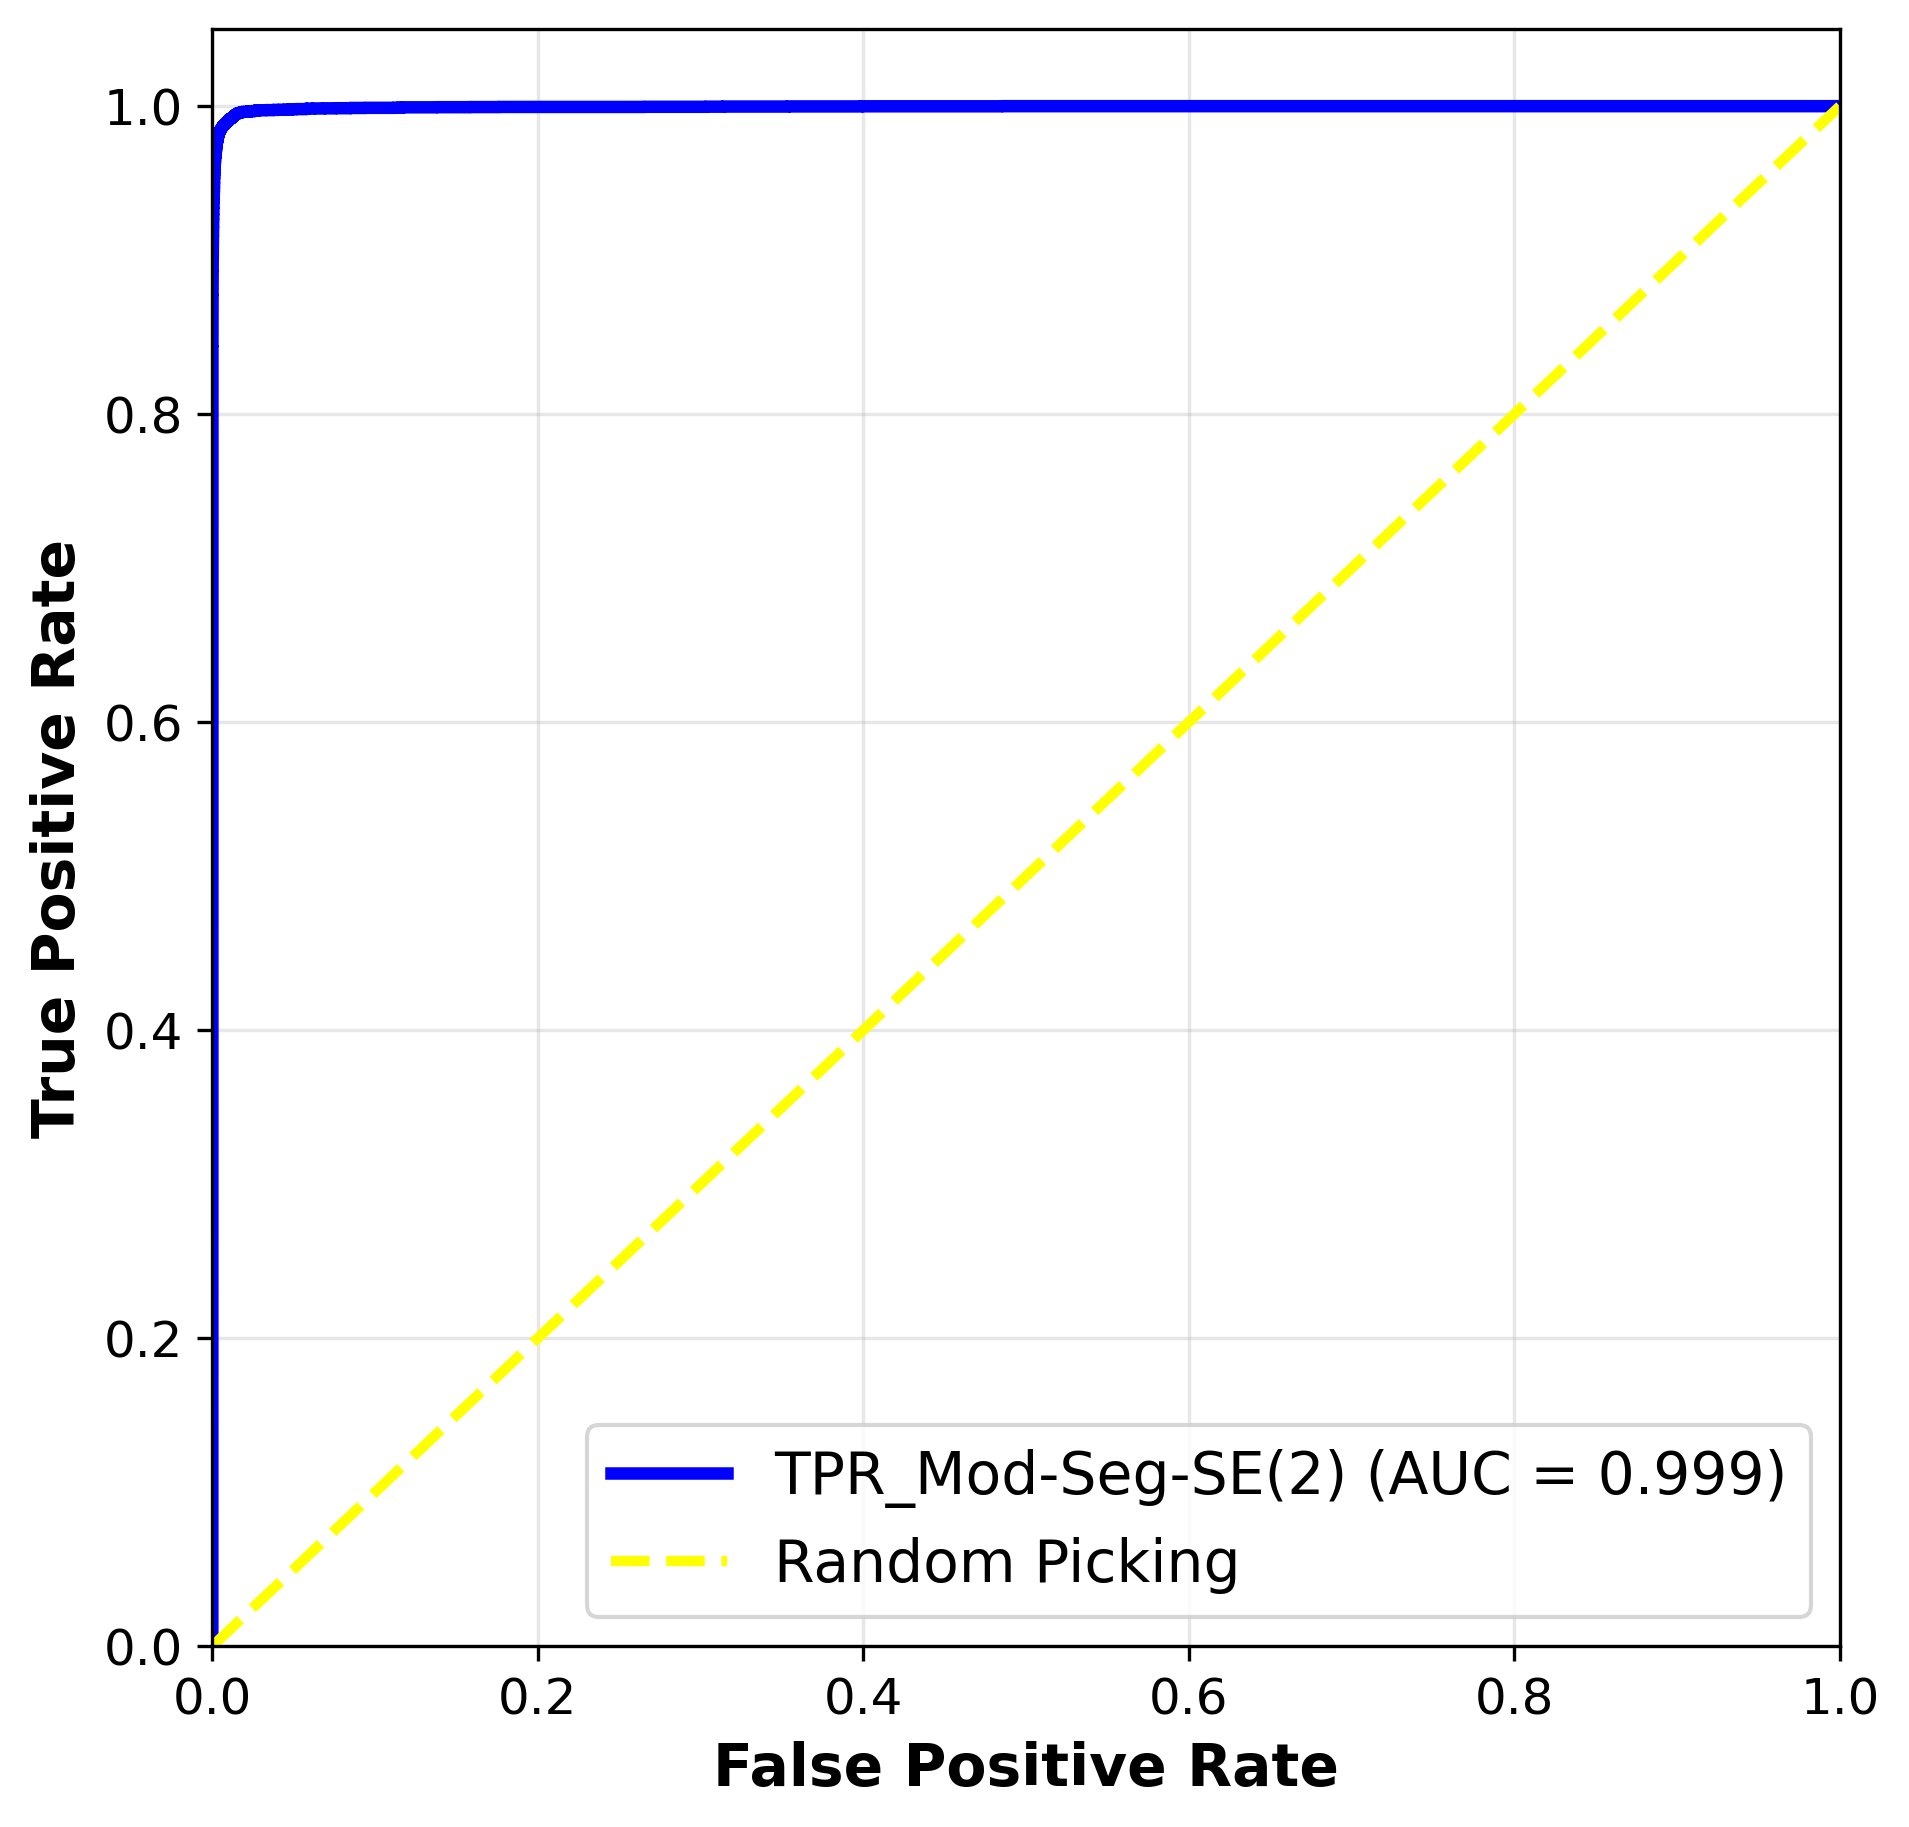
\includegraphics[width=\linewidth]{Journal_Figures/Fig3_Aggregated_ROC.png}
    \caption{Aggregated ROC curve demonstrating high classification performance across 10 folds, benefiting from the unified geometric framework.}
    \label{fig:roc}
\end{figure}

Finally, Figure~\ref{fig:multict} illustrates the consistency of our approach across multiple patients, further verifying that the 2.5D spatial context model effectively generalizes across varying anatomical structures and shapes without the need for exhaustive rotational data augmentation.

\begin{figure}[h]
    \centering
    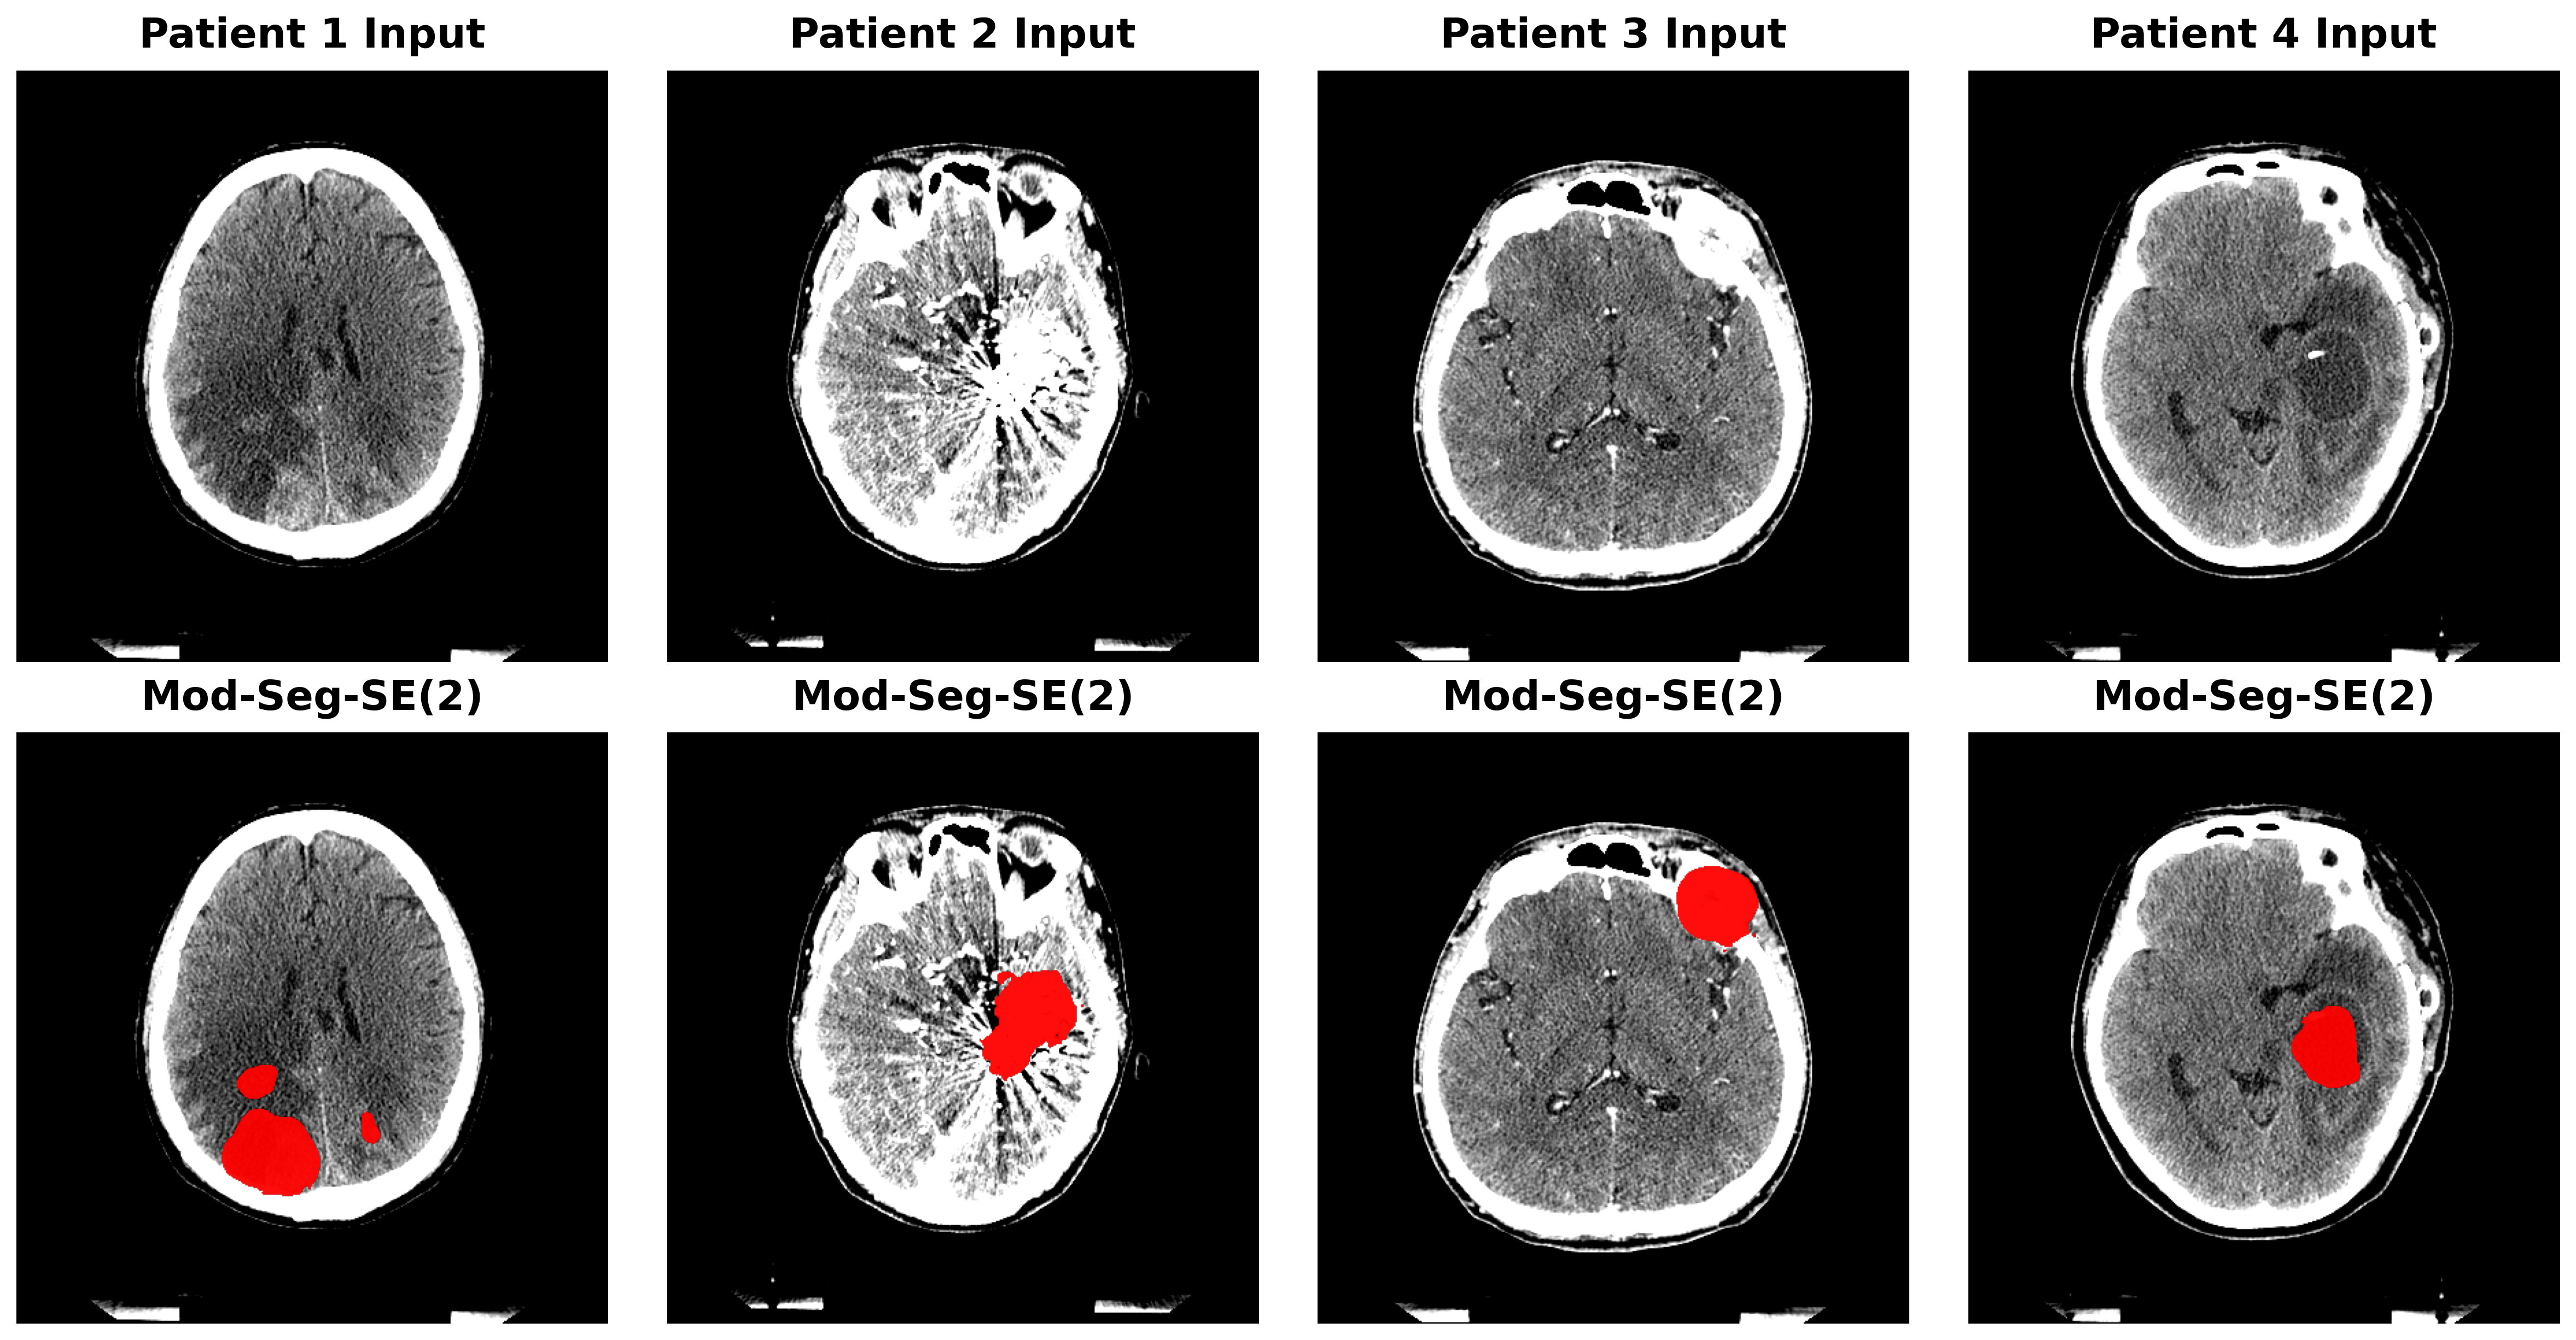
\includegraphics[width=\linewidth]{Journal_Figures/Fig4_Multi_CT_List.png}
    \caption{Extended multi-patient CT slice results indicating robust generalization across heterogeneous tumor morphologies.}
    \label{fig:multict}
\end{figure}

\subsection{Ablation Study}
To determine which components contribute most to performance gains, we systematically evaluated elements such as roto-translation equivariance, the 2.5D context logic, and the Edge-Boundary loss. The integration of the 2.5D context with roto-translation equivariance ensures that the model can robustly generalize across different spatial orientations across depth, leading to improved feature representation and decision-making over standard 2D baseline U-Nets.
